\documentclass[a4paper,12pt]{article}

\input{../../Preambulo.tex}
\newcommand{\assunto}{GEOMETRIA ANALÍTICA}
\newcommand{\atividade}{prova} % prova ou lista ou as ou ad ou atividade
\newcommand{\NumQObj}{5}
\newcommand{\NumQDisc}{1}
\pgfmathparse{int(\NumQObj + \NumQDisc)}
\edef\NumTotalQuestoes{\pgfmathresult}
\newcommand{\questaoDiscursiva}{Exercício \NumTotalQuestoes}
\newcommand{\ValorQObj}{1.4}
\newcommand{\ValorQDisc}{3}
\pgfmathparse{int(round(\NumQObj * \ValorQObj + \NumQDisc * \ValorQDisc))}
\edef\ValorProva{\pgfmathresult}
\newcommand{\tipo}{individual} % dupla ou individual
\newcommand{\calculadora}{nao} % sim ou nao
\newcommand{\turma}{INFORMÁTICA 3.\textordmasculine\ ANO}
\newcommand{\numProva}{A}
\newcommand{\professor}{Igor Martins Silva}
\newcommand{\bimestre}{2}
\newcommand{\ano}{2026}
\newcommand{\mesTexto}{junho}
\newcommand{\mesNum}{06}
\newcommand{\dia}{26}
\newcommand{\dataTexto}{\dia\ de \mesTexto\ de \ano}
\newcommand{\dataNun}{\dia/\mesNum/\ano}

\newcommand{\titulo}{}

\ifdefstring{\atividade}{prova}
  {\renewcommand{\titulo}{Avaliação de Matemática}}
{
\ifdefstring{\atividade}{lista}
  {\renewcommand{\titulo}{Lista de exercícios de Matemática}}
{
\ifdefstring{\atividade}{as}
  {\renewcommand{\titulo}{Avaliação Somativa}}
{
\ifdefstring{\atividade}{ad}
  {\renewcommand{\titulo}{Avaliação Diagnóstica}}
  {\renewcommand{\titulo}{Atividade de Matemática}}
}}}

\newcommand{\emtipo}{%
  \ifdefstring{\tipo}{individual}{\tipo}{em \tipo}%
}

\newcommand{\subtitulobase}[3]{%
    % #1 = título da 1ª coluna
    % #2 = conteúdo da 1ª coluna
    % #3 = mostra número da prova? (vazio ou algo)
    
    \begin{center}
        CEFET-MG -- Campus Contagem \\[3pt]
        \titulo\ -- \bimestre.\textordmasculine\ bimestre de \ano \\[3pt]
        \professor
    \end{center}
    
    \begin{center}
        \vspace{15pt}
        \begin{tabular}{|C{210pt}|C{70pt}|C{210pt}|}
            \hline
            \textbf{#1} &
            \textbf{DATA} &
            \textbf{TURMA} \\
            \hline
            #2 & \dataNun & \turma \\
            \hline
        \end{tabular}
    \end{center}
    
    #3
    
    \vspace{15pt}
}

\newcommand{\subtitulolis}{%
  \subtitulobase{ASSUNTO}{\assunto}{}%
}

\newcommand{\subtitulopr}{%
  \subtitulobase{ASSUNTO}{\assunto}{\boxed{\numProva}}%
}

\newcommand{\subtituloas}{%
  \subtitulobase{DISCIPLINA}{MATEMÁTICA}{}%
}

\newcommand{\subtituload}{%
  \subtitulobase{DISCIPLINA}{MATEMÁTICA}{}%
}

\newcommand{\valorquestao}{}

\newenvironment{exercicioBanco}[1][]{%
    \ifdefstring{\atividade}{prova}{%
        \begin{exercicio}[#1]%
    }{%
        \begin{exercicio}%
    }%
}{%
    \end{exercicio}
}

\ifdefstring{\atividade}{lista}{
    \pagecolor{background-color}
}{
    
}



\hypersetup{
    pdfauthor={\professor},
    pdftitle={\titulo \-- \assunto \-- \turma \-- \numProva},
}

\title{\titulo \-- \assunto \-- \turma \-- \numProva}
\author{\professor}
\date{\data}

%************* INÍCIO DO DOCUMENTO *************
\begin{document}
    \NoBgThispage
    \pagenumbering{alph}
    %
        
    \phantomsection
    \addcontentsline{toc}{section}{Capa}
    \input{../../PR_Capa}
    \newpage
        
    \phantomsection
    \addcontentsline{toc}{section}{Resposta para a questão discursiva}
    \input{../../RespQuestaoDisc}
    \addtocounter{page}{1}
    \newpage
    %
        
    \NoBgThispage
    \pagenumbering{arabic}
    %
        
    \subtitulopr
        
    %
    \begin{center}
        QUESTÕES OBJETIVAS
    \end{center}
    %
    
    \vspace{15pt}
    \newcommand{\modo}{objetivo} % objetivo ou discursivo
    
    \phantomsection
    \addcontentsline{toc}{section}{Exercício 1}
    %%%%%%%%%%%%%%%%%%%%%%%%%%%%%%%%%
%
%       EXERCÍCIO
%
%%%%%%%%%%%%%%%%%%%%%%%%%%%%%%%%%

\ifdefstring{\atividade}{prova}{%
    \ifdefstring{\modo}{objetivo}{%
        \renewcommand{\valorquestao}{\ValorQObj\ ponto}
    }{%
        \renewcommand{\valorquestao}{\ValorQDisc\ pontos}
    }%
}%

\begin{exercicioBanco}[\valorquestao]
Uma das extremidades de um segmento de reta é o ponto \(A = (1, 4)\). Sabendo que \(M = (5, 1)\) é o ponto médio desse segmento de reta, calcule as coordenadas do ponto \(B = (x, y)\), que é a outra extremidade do segmento de reta.

% Define as alternativas
\newcommand{\alternativas}{%
    \begin{center}
        \begin{tabularx}{\textwidth}{XXXXX}
            (a) \(x = 9\) e \(y = -2\). &
            (b) \(x = 8\) e \(y = -2\). &
            (c) \(x = 9\) e \(y = -1\). &
            (d) \(x = 7\) e \(y = -2\). &
            (e) \(x = 8\) e \(y = -1\).
        \end{tabularx}
    \end{center}
}

% Define a resposta correta
\newcommand{\resposta}{A}

% Lógica condicional para exibição
\ifdefstring{\atividade}{lista}{%
    \alternativas
    \vspace{0.5em}
    
    \noindent\textbf{Resposta:} letra \textbf{\resposta}.
}{%
    \ifdefstring{\modo}{objetivo}{%
        \alternativas
    }{%
        % modo = discursiva → não mostra alternativas
    }
}
\end{exercicioBanco}


    \vspace{15pt}
    
    \phantomsection
    \addcontentsline{toc}{section}{Exercício 2}
    %%%%%%%%%%%%%%%%%%%%%%%%%%%%%%%%%
%
%       EXERCÍCIO
%
%%%%%%%%%%%%%%%%%%%%%%%%%%%%%%%%%

\ifdefstring{\atividade}{prova}{%
    \ifdefstring{\modo}{objetivo}{%
        \renewcommand{\valorquestao}{\ValorQObj\ ponto}
    }{%
        \renewcommand{\valorquestao}{\ValorQDisc\ pontos}
    }%
}%

\begin{exercicioBanco}[\valorquestao]
Para cada afirmativa abaixo, assinale se ela é verdadeira (V) ou falsa (F).
%
\begin{enumerate}[\(\bullet\)]
    \item \(A = (1,2)\), \(B = (3,6)\) e \(C = (5,10)\) estão alinhados.
    %
    \item As retas \(r\) e \(s\) determinadas, respectivamente, pelas equações \(6x + 9y - 3 = 0\) e \(2x + 3y + 5 = 0\) são paralelas.
    %
    \item A distância entre o ponto \(P = (1,2)\) e a reta \(r: 3x + 4y - 10 = 0\) é \(1\).
\end{enumerate}
%

% Define as alternativas
\newcommand{\alternativas}{%
    \begin{center}
        \begin{tabularx}{\textwidth}{XXXXX}
            (a) (V, V, V). &
            (b) (V, V, F). &
            (c) (F, V, F). &
            (d) (V, F, V). &
            (e) (F, V, V).
        \end{tabularx}
    \end{center}
}

% Define a resposta correta
\newcommand{\resposta}{B}

% Lógica condicional para exibição
\ifdefstring{\atividade}{lista}{%
    \alternativas
    \vspace{0.5em}
    
    \noindent\textbf{Resposta:} letra \textbf{\resposta}.
}{%
    \ifdefstring{\modo}{objetivo}{%
        \alternativas
    }{%
        % modo = discursiva → não mostra alternativas
    }
}
\end{exercicioBanco}


    \vspace{15pt}
    
    \phantomsection
    \addcontentsline{toc}{section}{Exercício 3}
    %%%%%%%%%%%%%%%%%%%%%%%%%%%%%%%%%
%
%       EXERCÍCIO
%
%%%%%%%%%%%%%%%%%%%%%%%%%%%%%%%%%

\ifdefstring{\atividade}{prova}{%
    \ifdefstring{\modo}{objetivo}{%
        \renewcommand{\valorquestao}{\ValorQObj\ ponto}
    }{%
        \renewcommand{\valorquestao}{\ValorQDisc\ pontos}
    }%
}%

\begin{exercicioBanco}[\valorquestao]
No plano cartesiano representado abaixo, as retas \(r\) e \(s\) são perpendiculares. Determine a área da região destacada, em alguma unidade de área (u.a.).

\begin{center}
    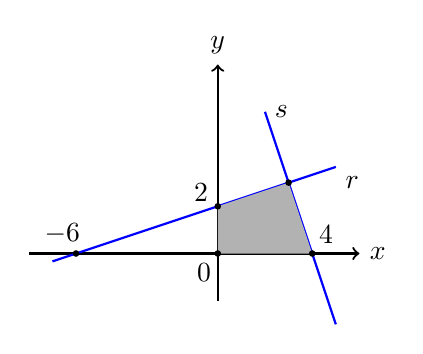
\begin{tikzpicture}[scale=0.3]
        % Eixos
        \draw[->,thick] (-8,0) -- (6,0) node[right] {$x$};
        \draw[->,thick] (0,-2) -- (0,8) node[above] {$y$};

        % Retas
        \draw[domain=-7:5, smooth, variable=\x, blue, thick] 
        plot ({\x}, {\x/3+2});
        
        \draw[domain=2:5, smooth, variable=\x, blue, thick] 
        plot ({\x}, {-3*\x+12});

        % Quadrilátero sombreado
        \fill[gray!60]
        (0,0) --
        (0,2) --
        (3,3) --
        (4,0) -- cycle;

        % Marcas no eixo x
        \node[left, above, xshift=-5pt] at (-6,0) {$-6$};
        \node[left, below, xshift=-5pt] at (0,0) {$0$};
        \node[right, above, xshift=5pt] at (4,0) {$4$};

        % Marca no eixo y
        \node[left,yshift=5pt] at (0,2) {$2$};

        % Identificação das retas
        \node[right] at (5,3) {$r$};
        \node[right] at (2,6) {$s$};
        
        % Pontos importantes
        \fill (0,0) circle (4pt);
        \fill (0,2) circle (4pt);
        \fill (3,3) circle (4pt);
        \fill (4,0) circle (4pt);
        \fill (-6,0) circle (4pt);
    \end{tikzpicture}
\end{center}

% Define as alternativas
\newcommand{\alternativas}{%
    \begin{center}
        \begin{tabularx}{\textwidth}{XXXXX}
            (a) 8 u.a.. &
            (b) 9 u.a.. &
            (c) 10 u.a.. &
            (d) 11 u.a.. &
            (e) 12 u.a..
        \end{tabularx}
    \end{center}
}

% Define a resposta correta
\newcommand{\resposta}{B}

% Lógica condicional para exibição
\ifdefstring{\atividade}{lista}{%
    \alternativas
    \vspace{0.5em}
    
    \noindent\textbf{Resposta:} letra \textbf{\resposta}.
}{%
    \ifdefstring{\modo}{objetivo}{%
        \alternativas
    }{%
        % modo = discursiva → não mostra alternativas
    }
}
\end{exercicioBanco}


    \vspace{15pt}
    
    \phantomsection
    \addcontentsline{toc}{section}{Exercício 4}
    %%%%%%%%%%%%%%%%%%%%%%%%%%%%%%%%%
%
%       EXERCÍCIO
%
%%%%%%%%%%%%%%%%%%%%%%%%%%%%%%%%%

\ifdefstring{\atividade}{prova}{%
    \ifdefstring{\modo}{objetivo}{%
        \renewcommand{\valorquestao}{\ValorQObj\ ponto}
    }{%
        \renewcommand{\valorquestao}{\ValorQDisc\ pontos}
    }%
}%

\begin{exercicioBanco}[\valorquestao]
Em relação às circunferência \(C_{1}: x^{2} + y^{2} - 2x - 2y - 8 = 0\) e \(C_{2}: x^{2} + y^{2} + 10x + 2y + 16 = 0\), é correto afirmar que são:

% Define as alternativas
\newcommand{\alternativas}{%
    \begin{center}
        \begin{tabularx}{\textwidth}{XXX}
            (a) exteriores. &
            (b) tangentes exteriormente. &
            (c) secantes. \\[5pt]
            (d) tangentes interiormente. &
            (e) interiores.
        \end{tabularx}
    \end{center}
}

% Define a resposta correta
\newcommand{\resposta}{B}

% Lógica condicional para exibição
\ifdefstring{\atividade}{lista}{%
    \alternativas
    \vspace{0.5em}
    
    \noindent\textbf{Resposta:} letra \textbf{\resposta}.
}{%
    \ifdefstring{\modo}{objetivo}{%
        \alternativas
    }{%
        % modo = discursiva → não mostra alternativas
    }
}
\end{exercicioBanco}


    \vspace{15pt}
    
    \phantomsection
    \addcontentsline{toc}{section}{Exercício 5}
    %%%%%%%%%%%%%%%%%%%%%%%%%%%%%%%%%
%
%       EXERCÍCIO
%
%%%%%%%%%%%%%%%%%%%%%%%%%%%%%%%%%

\ifdefstring{\atividade}{prova}{%
    \ifdefstring{\modo}{objetivo}{%
        \renewcommand{\valorquestao}{\ValorQObj\ ponto}
    }{%
        \renewcommand{\valorquestao}{\ValorQDisc\ pontos}
    }%
}%

\begin{exercicioBanco}[\valorquestao]
Em relação às circunferências \(C_{1}: x^{2} + y^{2} - 4x - 6y + 9 = 0\) e \(C_{2}: x^{2} + y^{2} + 2x + 2y - 11 = 0\), é correto afirmar que são:

% Define as alternativas
\newcommand{\alternativas}{%
    \begin{center}
        \begin{tabularx}{\textwidth}{XXX}
            (a) exteriores. &
            (b) tangentes exteriormente. &
            (c) secantes. \\[5pt]
            (d) tangentes interiormente. &
            (e) interiores.
        \end{tabularx}
    \end{center}
}

% Define a resposta correta
\newcommand{\resposta}{C}

% Lógica condicional para exibição
\ifdefstring{\atividade}{lista}{%
    \alternativas
    \vspace{0.5em}
    
    \noindent\textbf{Resposta:} letra \textbf{\resposta}.
}{%
    \ifdefstring{\modo}{objetivo}{%
        \alternativas
    }{%
        % modo = discursiva → não mostra alternativas
    }
}
\end{exercicioBanco}


    \vspace{15pt}
    
    %
    \begin{center}
        QUESTÃO DISCURSIVA 
    \end{center}
    %
    \vspace{15pt}
    
    \renewcommand{\modo}{discursivo} % objetivo ou discursivo
    \phantomsection
    \addcontentsline{toc}{section}{Exercício 6}
    %%%%%%%%%%%%%%%%%%%%%%%%%%%%%%%%%
%
%       EXERCÍCIO
%
%%%%%%%%%%%%%%%%%%%%%%%%%%%%%%%%%

\ifdefstring{\atividade}{prova}{%
    \ifdefstring{\modo}{objetivo}{%
        \renewcommand{\valorquestao}{\ValorQObj\ ponto}
    }{%
        \renewcommand{\valorquestao}{\ValorQDisc\ pontos}
    }%
}%

\begin{exercicioBanco}[\valorquestao]
Três cidades \(A\), \(B\) e \(C\) situam-se ao longo de uma estrada reta; \(B\) situa-se entre \(A\) e \(C\) e a distância de \(B\) a \(C\) é igual à metade da distância de \(A\) a \(B\). Um encontro foi marcado por 3 moradores, um de cada cidade, em um ponto \(P\) da estrada, localizado entre as cidades \(B\) e \(C\) e à distância de 180 km de \(A\). Sabendo-se que \(P\) está 30 km mais próximo de \(C\) do que de \(B\), determinar a distância que o morador de \(B\) deverá percorrer até o ponto de encontro.

% Define as alternativas
\newcommand{\alternativas}{%
    \begin{center}
        \begin{tabularx}{\textwidth}{XXXXX}
            (a) \(30\) km. &
            (b) \(40\) km. &
            (c) \(50\) km. &
            (d) \(60\) km. &
            (e) \(70\) km.
        \end{tabularx}
    \end{center}
}

% Define a resposta correta
\newcommand{\resposta}{D}

% Lógica condicional para exibição
\ifdefstring{\atividade}{lista}{%
    \alternativas
    \vspace{0.5em}
    
    \noindent\textbf{Resposta:} letra \textbf{\resposta}.
}{%
    \ifdefstring{\modo}{objetivo}{%
        \alternativas
    }{%
        % modo = discursiva → não mostra alternativas
    }
}
\end{exercicioBanco}


    \vspace{10pt}
    
    %\newpage
    
    %\phantomsection
    %\addcontentsline{toc}{section}{Rascunho}
    %\input{../../Rascunho}
    
\end{document}
%*************** FINAL DO DOCUMENTO ***************
